%*************************************
% ภาคผนวก ง.
%*************************************
\vspace{-0.5in}

\appendixChapterTitle{ง}{คู่มือการใช้งานแพลตฟอร์ม (Platform Usage)}

\section{การเริ่มต้นใช้งาน}
\hspace*{1.3em}
ภาคผนวกนี้สรุปขั้นตอนการใช้งาน FITM Cloud ผ่านหน้า Dashboard (Midori) สำหรับผู้ใช้งานทุกบทบาท (Student / Instructor / Admin) โดยเน้นลำดับการใช้งานแบบรวดเร็วและกรณีที่พบบ่อย

\begin{mycustomenum2}
    \item เข้าสู่ระบบที่ \textbf{/login}
    \item ไปที่ \textbf{Dashboard \textrightarrow Settings} เพื่อตรวจสอบ \textbf{Role} ของบัญชี
    \item ใน \textbf{Settings \textrightarrow SSH Keys} เพิ่ม SSH public key อย่างน้อย 1 key
    \item (Student) ไปที่ \textbf{Dashboard \textrightarrow Requests \textrightarrow New Request} เพื่อส่งคำขอสร้าง instance
    \item เมื่อคำขอได้รับอนุมัติและ provision เสร็จ ให้ไปที่ \textbf{Dashboard \textrightarrow Instances} เลือก instance แล้วใช้ \textbf{IP address} เพื่อเชื่อมต่อด้วย SSH
\end{mycustomenum2}

\begin{figure}[H]
\centering
\adjustbox{frame, width=0.9\textwidth}{
    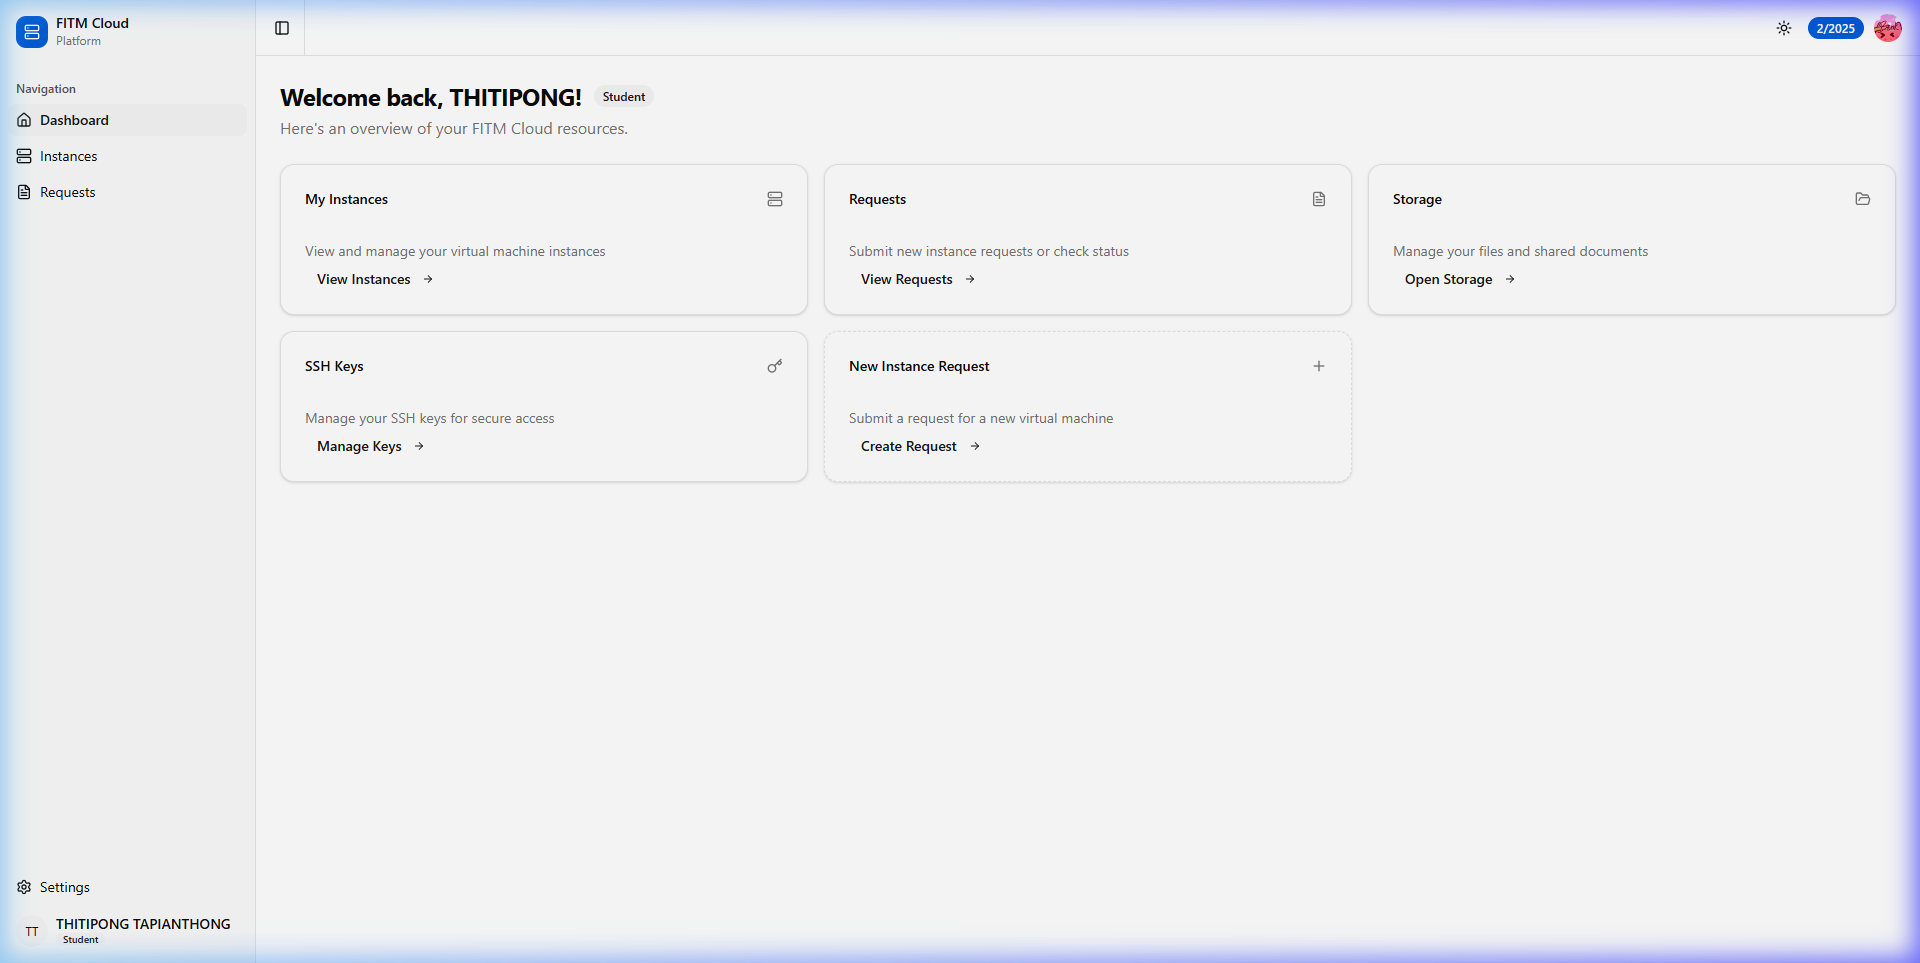
\includegraphics[width=\textwidth]{Image/web/dashboard/student_captured/student_dashboard.png}
}
\caption{\fontSixTeen{ภาพหน้าจอแดชบอร์ดหลักและขั้นตอนเริ่มต้นใช้งานแพลตฟอร์ม}}
\label{figI:StartPlaceholder}
\end{figure}

\section{ขั้นตอนการใช้งานสำหรับนักศึกษา}
\hspace*{1.3em}
การทำงานหลักของนักศึกษาคือการส่งคำขอสร้าง instance ติดตามสถานะ และใช้งาน instance ที่ได้รับการ provision

\vspace{0.5em}
\textbf{Create a new VM request}
\vspace{0.5em}

\begin{figure}[H]
\centering
\adjustbox{frame, width=0.9\textwidth}{
    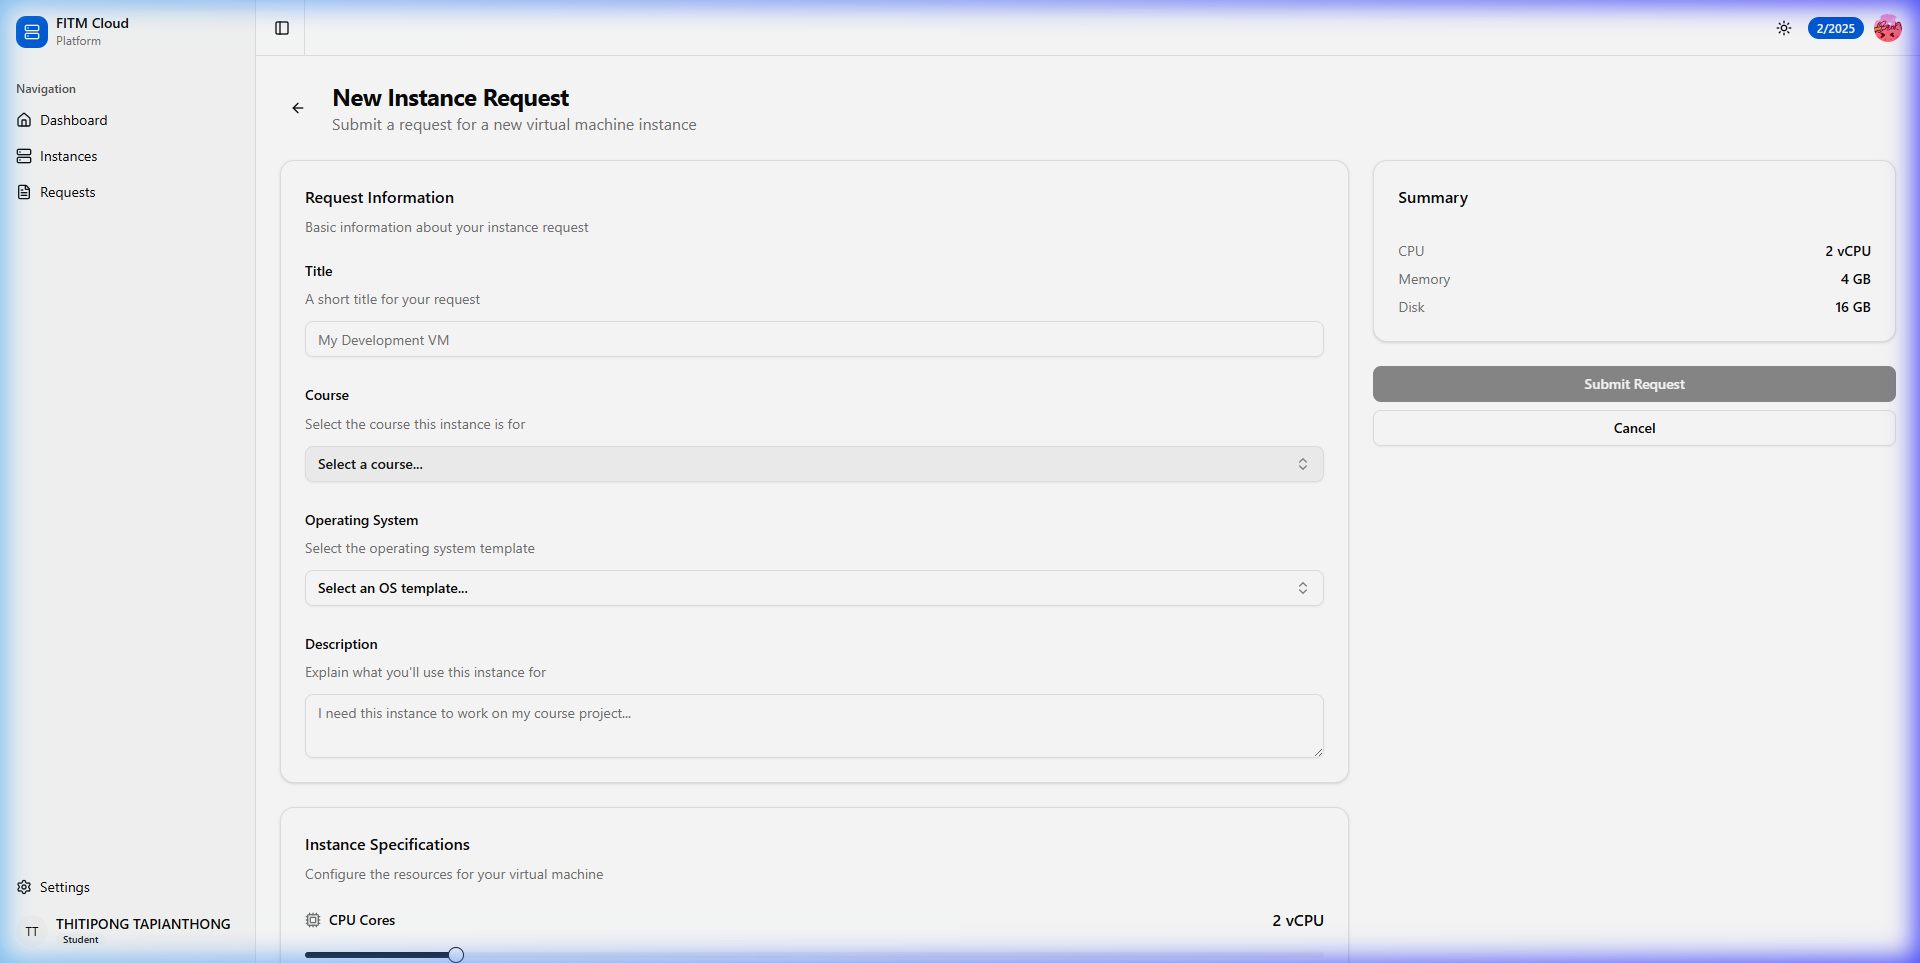
\includegraphics[width=\textwidth]{Image/web/dashboard/student_captured/student_new_request.png}
}
\caption{\fontSixTeen{ภาพหน้าจอแบบฟอร์มการสร้างคำร้องขอเครื่องเสมือนใหม่ (New Request)}}
\label{figI:StudentRequestPlaceholder}
\end{figure}

\begin{mycustomenum2}
    \item ไปที่ \textbf{Dashboard \textrightarrow Requests \textrightarrow New Request}
    \item กรอกข้อมูลหลัก:
    \begin{mycustomenum2}
        \item \textbf{Title} ชื่อสั้น ๆ ของคำขอ
        \item \textbf{Course} รายวิชา/ภาคการศึกษาที่เกี่ยวข้อง
        \item \textbf{Operating System} (template)
        \item \textbf{Description} อธิบายวัตถุประสงค์การใช้งาน
        \item \textbf{CPU / Memory / Disk} ตามความต้องการ
    \end{mycustomenum2}
    \item กด \textbf{Submit Request}
\end{mycustomenum2}

\vspace{0.5em}
\textbf{Track request status}
\vspace{0.5em}

\begin{figure}[H]
\centering
\adjustbox{frame, width=0.9\textwidth}{
    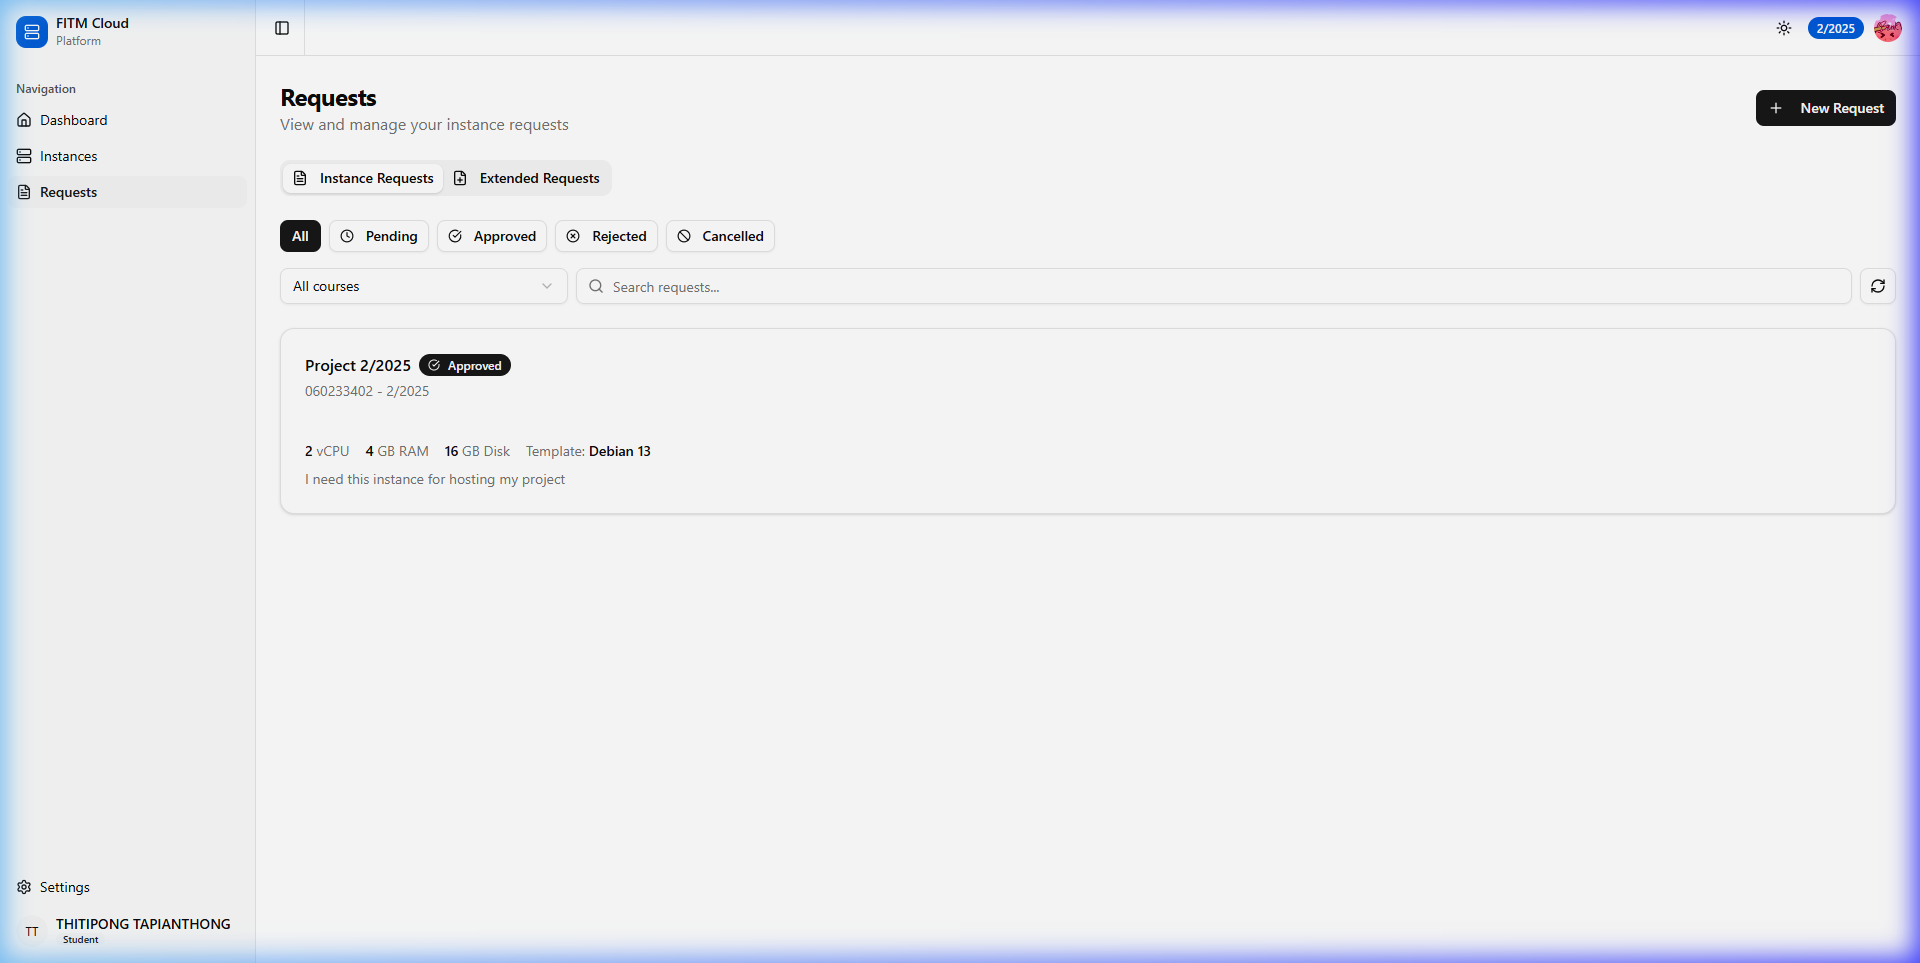
\includegraphics[width=\textwidth]{Image/web/dashboard/student_captured/student_requests_list.png}
}
\caption{\fontSixTeen{ภาพหน้าจอรายการคำร้องขอเครื่องเสมือนและสถานะการดำเนินการ}} 
\label{figI:StudentStatusPlaceholder}
\end{figure}

\begin{mycustomenum2}
    \item ไปที่ \textbf{Dashboard \textrightarrow Requests}
    \item ความหมายสถานะ:
    \begin{mycustomenum2}
        \item \textbf{Pending}: รอการพิจารณา
        \item \textbf{Approved}: อนุมัติแล้ว (กำลัง provision หรือ provision แล้ว)
        \item \textbf{Rejected}: ไม่อนุมัติ
        \item \textbf{Cancelled}: ยกเลิกโดยระบบหรือผู้พิจารณา
    \end{mycustomenum2}
\end{mycustomenum2}

\vspace{0.5em}
\textbf{Use your VM}
\vspace{0.5em}

\begin{figure}[H]
\centering
\adjustbox{frame, width=0.9\textwidth}{
    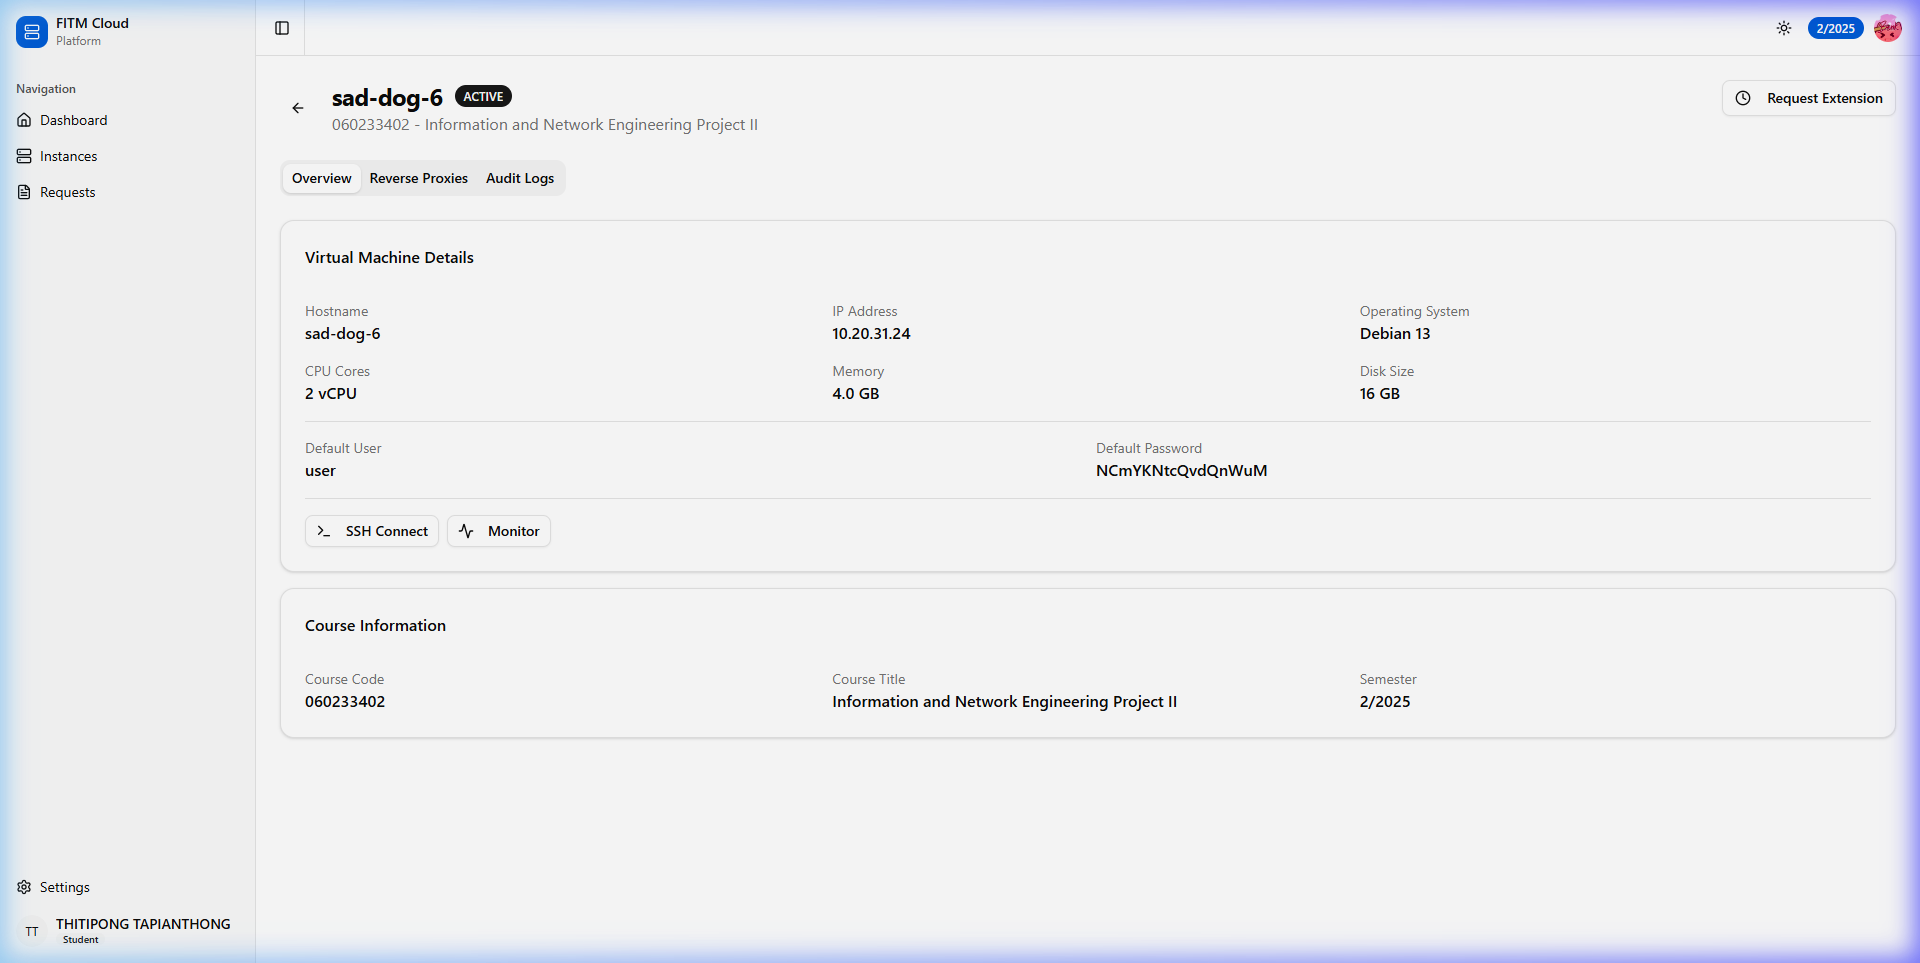
\includegraphics[width=\textwidth]{Image/web/dashboard/student_captured/student_instance.png}
}
\caption{\fontSixTeen{ภาพหน้าจอดูรายละเอียดและสถานะของเครื่องเสมือน (Instance Overview)}} 
\label{figI:StudentInstancePlaceholder}
\end{figure}

\begin{mycustomenum2}
    \item ไปที่ \textbf{Dashboard \textrightarrow Instances} แล้วเลือก instance
    \item ในหน้า \textbf{Overview} ตรวจสอบ \textbf{IP Address} และ \textbf{Hostname}
    \item เชื่อมต่อด้วย SSH ตามหัวข้อ \textbf{SSH \& Access}
\end{mycustomenum2}

\vspace{0.5em}
\textbf{Request more time (extension request)}
\vspace{0.5em}

\begin{figure}[H]
\centering
\adjustbox{frame, width=0.9\textwidth}{
    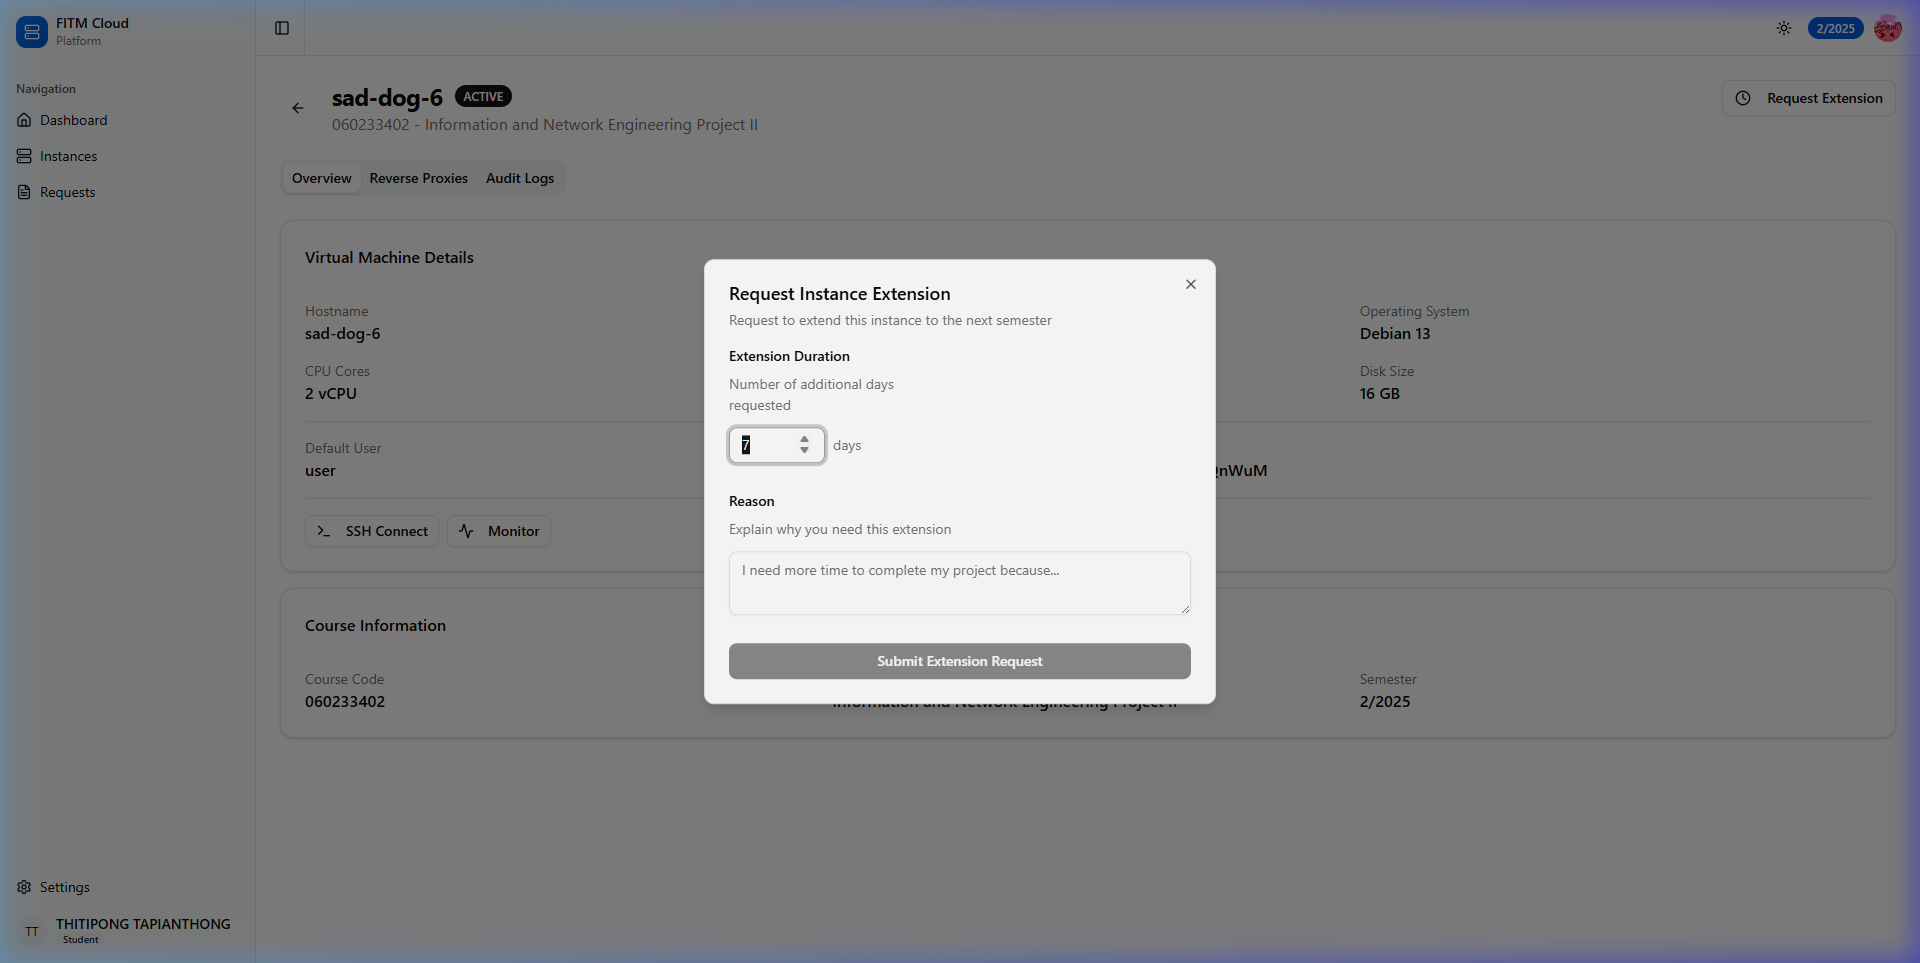
\includegraphics[width=\textwidth]{Image/web/dashboard/student_captured/student_extension.png}
}
\caption{\fontSixTeen{ภาพหน้าจอการขอขยายเวลาการใช้งาน Instance (Extension Request)}} 
\label{figI:StudentExtension}
\end{figure}

\begin{mycustomenum2}
    \item ไปที่ \textbf{Dashboard \textrightarrow Instances} แล้วเลือก instance
    \item ใช้เมนู \textbf{Extension Request} (หาก role อนุญาต)
    \item ระบุจำนวนวันและเหตุผล
    \item ติดตามสถานะที่ \textbf{Dashboard \textrightarrow Requests \textrightarrow Extended}
\end{mycustomenum2}

\begin{figure}[H]
\centering
\adjustbox{frame, width=0.9\textwidth}{
    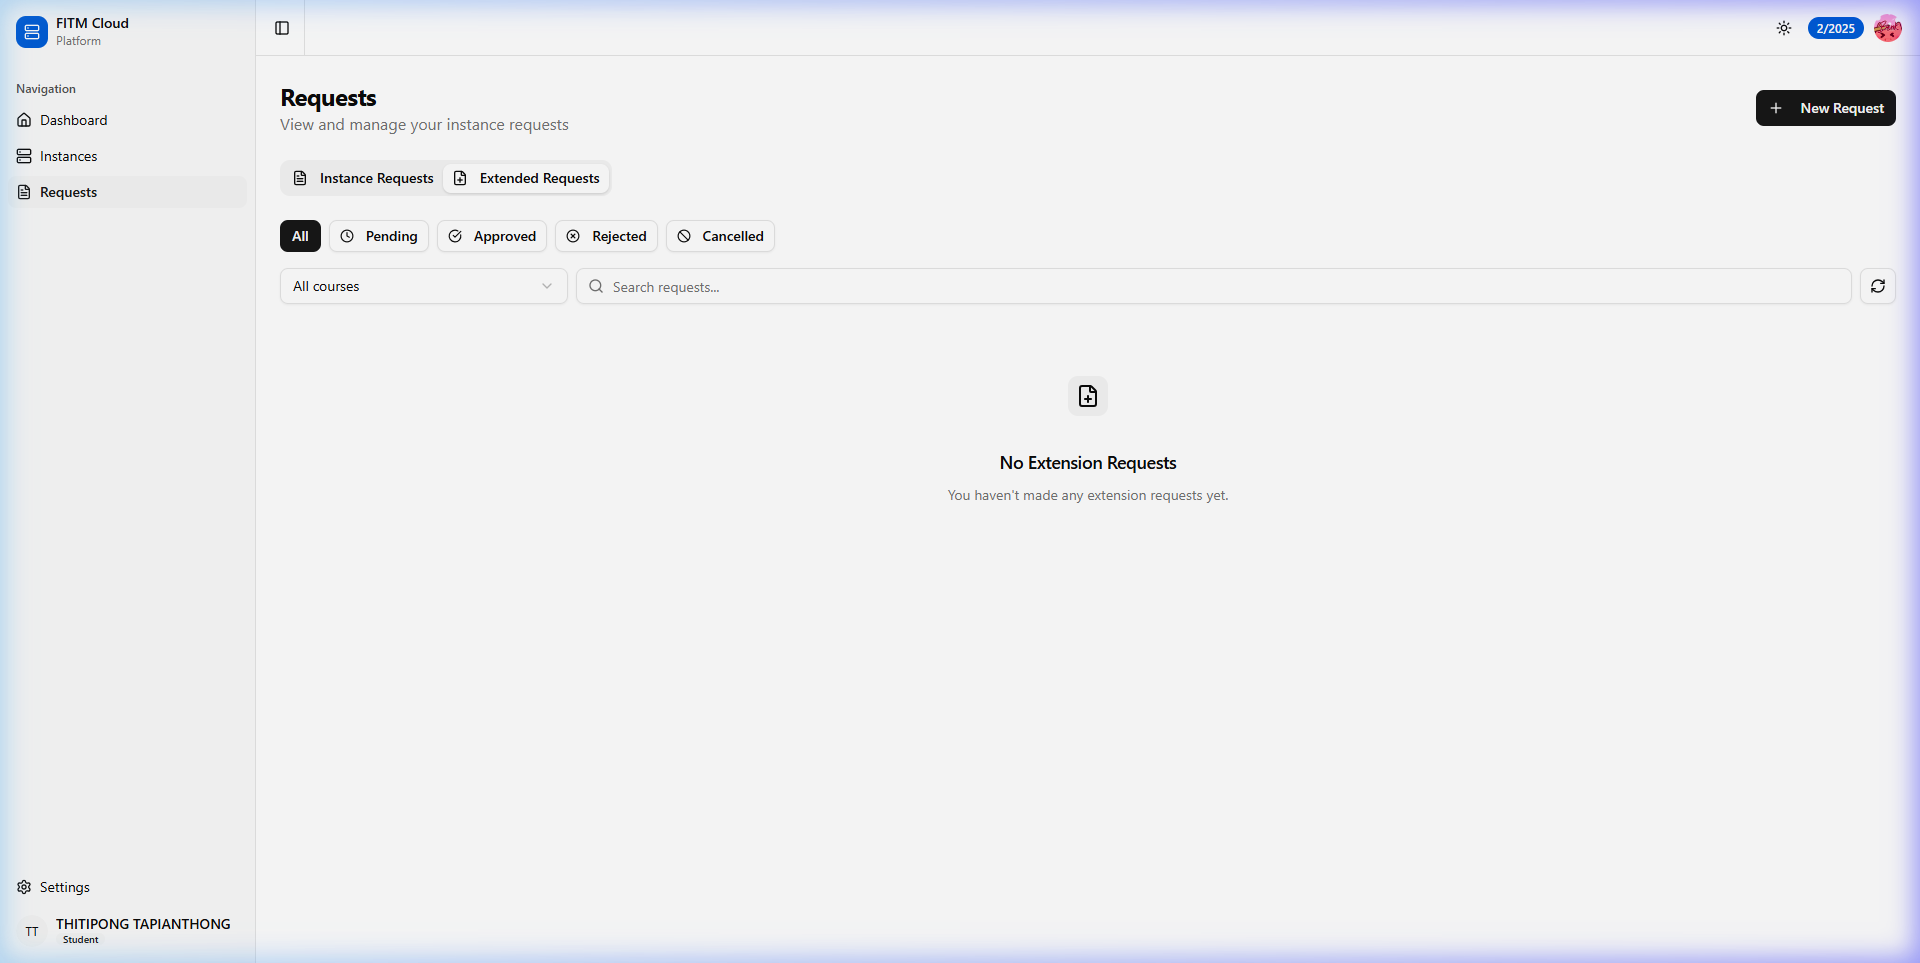
\includegraphics[width=\textwidth]{Image/web/dashboard/student_captured/student_extended_list.png}
}
\caption{\fontSixTeen{ภาพหน้าจอรายการคำขอขยายเวลา (Extended Requests)}} 
\label{figI:StudentExtendedList}
\end{figure}

\section{ขั้นตอนการใช้งานสำหรับผู้สอน}
\hspace*{1.3em}
ผู้สอนมีหน้าที่หลักในการพิจารณาคำขอของนักศึกษา และจัดการ instance ที่เกี่ยวข้องกับรายวิชา

\vspace{0.5em}
\textbf{Review incoming requests}
\vspace{0.5em}

\begin{figure}[H]
\centering
\adjustbox{frame, width=0.9\textwidth}{
    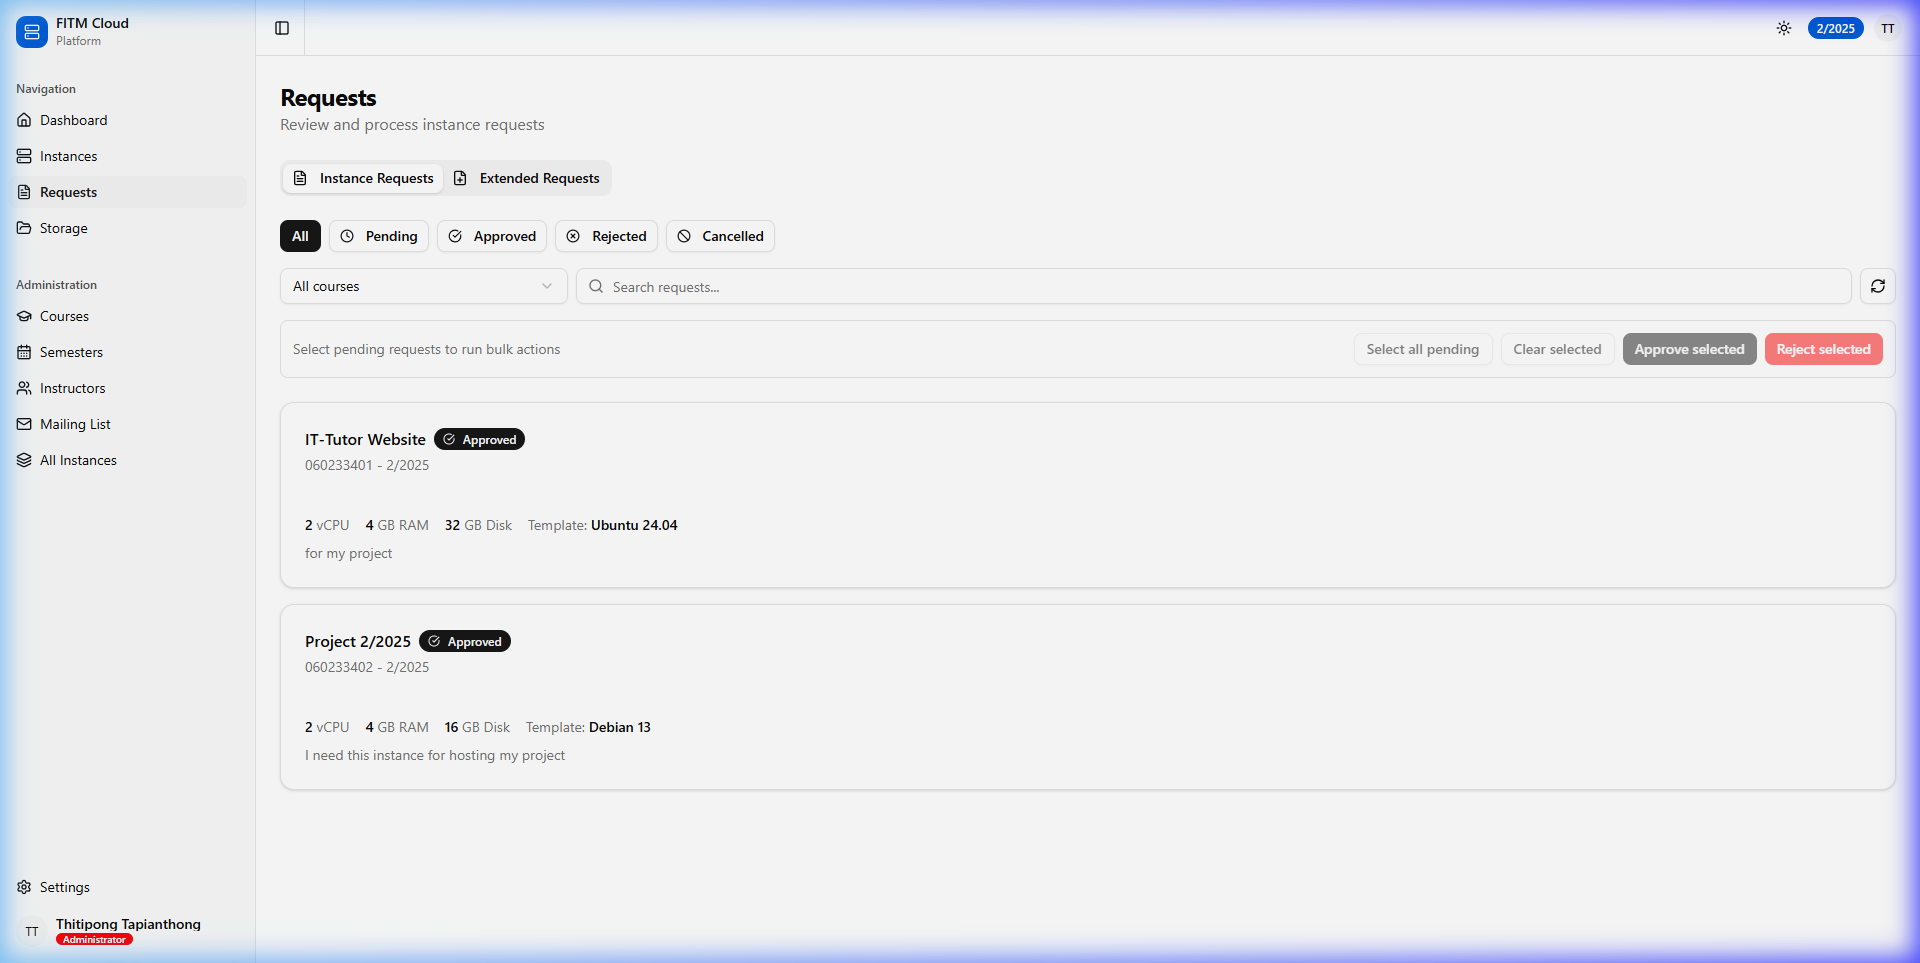
\includegraphics[width=\textwidth]{Image/web/dashboard/captured/requests_list.png}
}
\caption{\fontSixTeen{ภาพหน้าจอการพิจารณาและอนุมัติคำร้องขอเครื่องเสมือนสำหรับผู้สอน}} 
\label{figI:InstructorReviewPlaceholder}
\end{figure}

\begin{mycustomenum2}
    \item ไปที่ \textbf{Dashboard \textrightarrow Requests}
    \item ตรวจสอบรายการที่เป็น \textbf{Pending} และเลือก \textbf{Approve} หรือ \textbf{Reject}
    \item สามารถปรับสเปคก่อนอนุมัติได้:
    \begin{mycustomenum2}
        \item ปรับทีละรายการด้วย \textbf{Edit specs}
        \item หรือปรับแบบกลุ่มด้วยตัวเลือก \textbf{Modify specs} ในส่วน bulk actions
    \end{mycustomenum2}
\end{mycustomenum2}

\vspace{0.5em}
\textbf{Manage instances}
\vspace{0.5em}

\begin{mycustomenum2}
    \item ไปที่ \textbf{Dashboard \textrightarrow Instances}
    \item ใช้ \textbf{Promote} สำหรับ instance ที่ต้องเป็น long-term (ตามนโยบายรายวิชา)
    \item ใช้ \textbf{Audit Logs} ในหน้ารายละเอียด instance เพื่อดูประวัติการเปลี่ยนแปลง
\end{mycustomenum2}

\vspace{0.5em}
\textbf{Review extension requests}
\vspace{0.5em}

\begin{mycustomenum2}
    \item ไปที่ \textbf{Dashboard \textrightarrow Requests \textrightarrow Extended}
    \item พิจารณาและเลือกอนุมัติ/ปฏิเสธตามนโยบาย
\end{mycustomenum2}

\section{ขั้นตอนการใช้งานสำหรับผู้ดูแลระบบ}
\hspace*{1.3em}
ผู้ดูแลระบบใช้งานเมนู Admin เพื่อจัดการข้อมูลวิชาการและบัญชีผู้สอน รวมถึงตรวจสอบภาพรวมของ instance ทั้งระบบ

\begin{figure}[H]
\centering
\adjustbox{frame, width=0.9\textwidth}{
    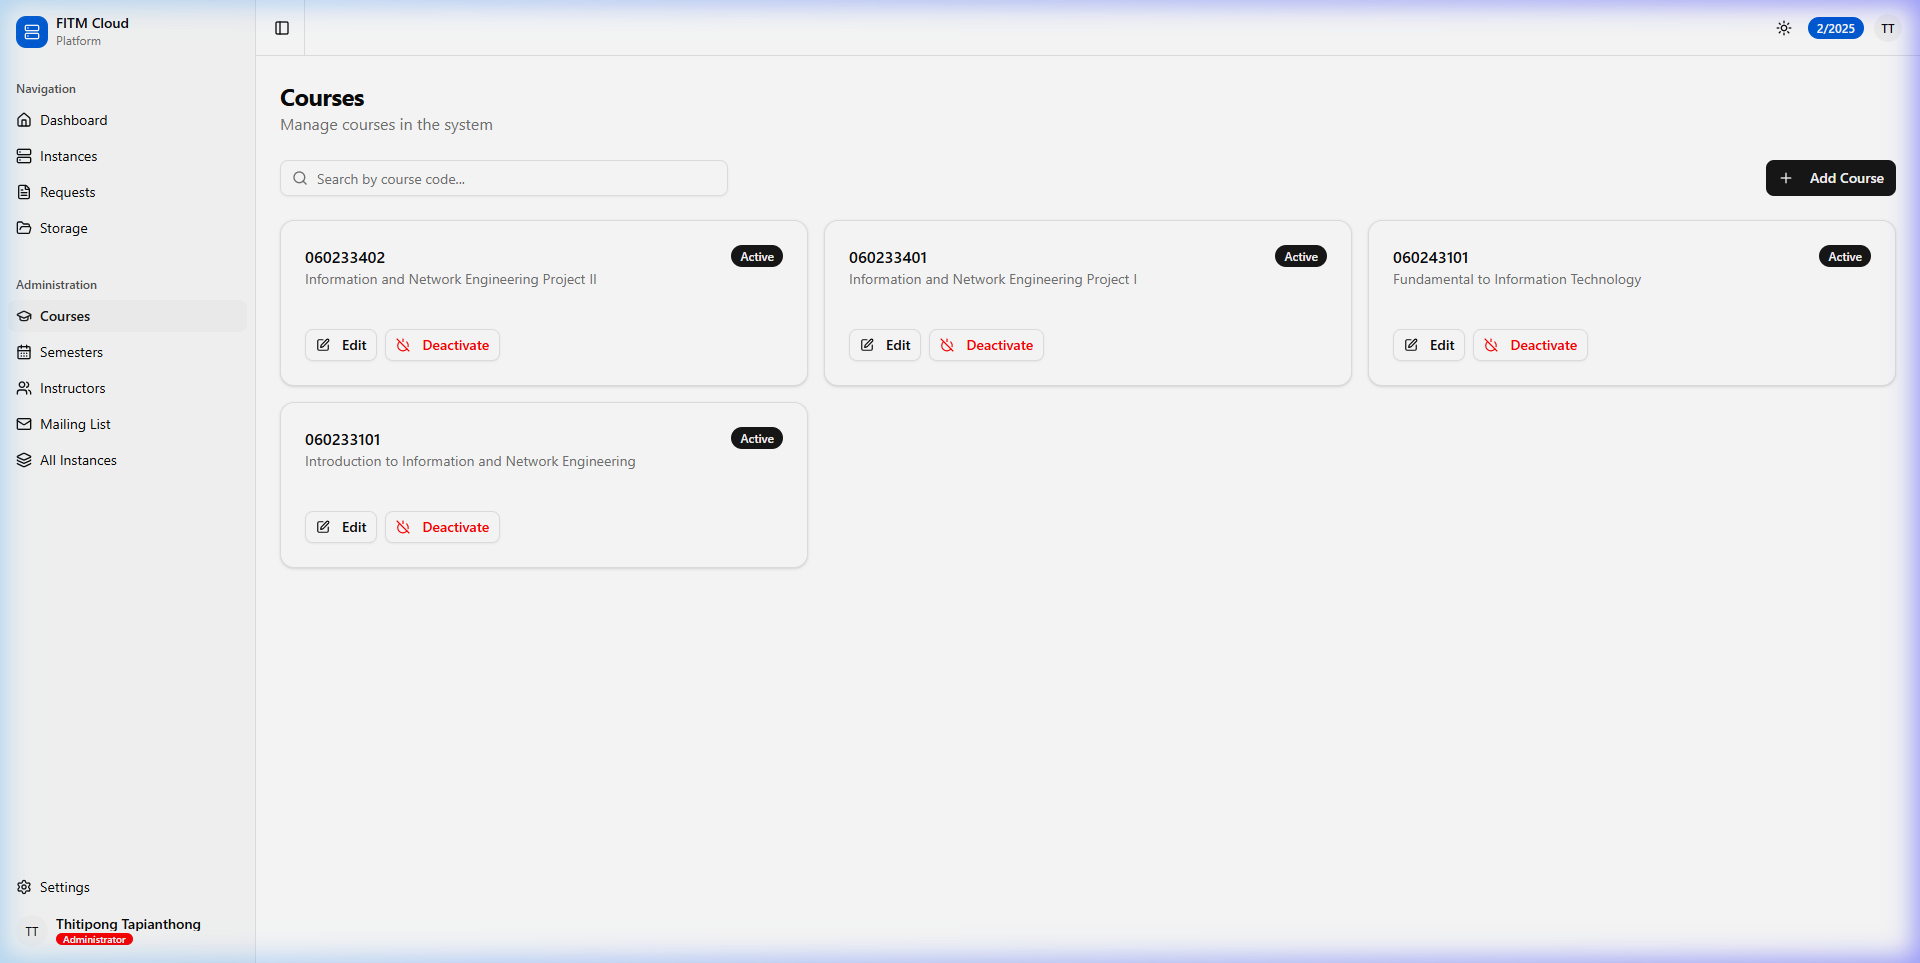
\includegraphics[width=\textwidth]{Image/web/dashboard/captured/admin_menu.png}
}
\caption{\fontSixTeen{ภาพหน้าจอเมนูผู้ดูแลระบบและการจัดการข้อมูลวิชาการ}} 
\label{figI:AdminPlaceholder}
\end{figure}

\begin{mycustomenum2}
    \item ไปที่ \textbf{Dashboard \textrightarrow Admin}
    \item งานที่พบบ่อย:
    \begin{mycustomenum2}
        \item \textbf{Courses}: สร้าง/แก้ไขรายวิชา
        \item \textbf{Semesters}: จัดการภาคการศึกษาและตั้งค่าภาคปัจจุบัน
        \item \textbf{Instructors}: จัดการบัญชีผู้สอน
        \item \textbf{Mailing List}: จัดการรายการรับข่าวสาร
        \item \textbf{Instances}: ตรวจสอบ instance ทั้งระบบ
    \end{mycustomenum2}
\end{mycustomenum2}

\section{การเข้าถึงด้วย SSH}
\hspace*{1.3em}
การเข้าถึง instance ใช้ SSH เป็นหลัก โดยแนะนำให้ใช้ SSH keys แทนรหัสผ่าน

\vspace{0.5em}
\textbf{Add your SSH key}
\vspace{0.5em}

\begin{figure}[H]
\centering
\adjustbox{frame, width=0.9\textwidth}{
    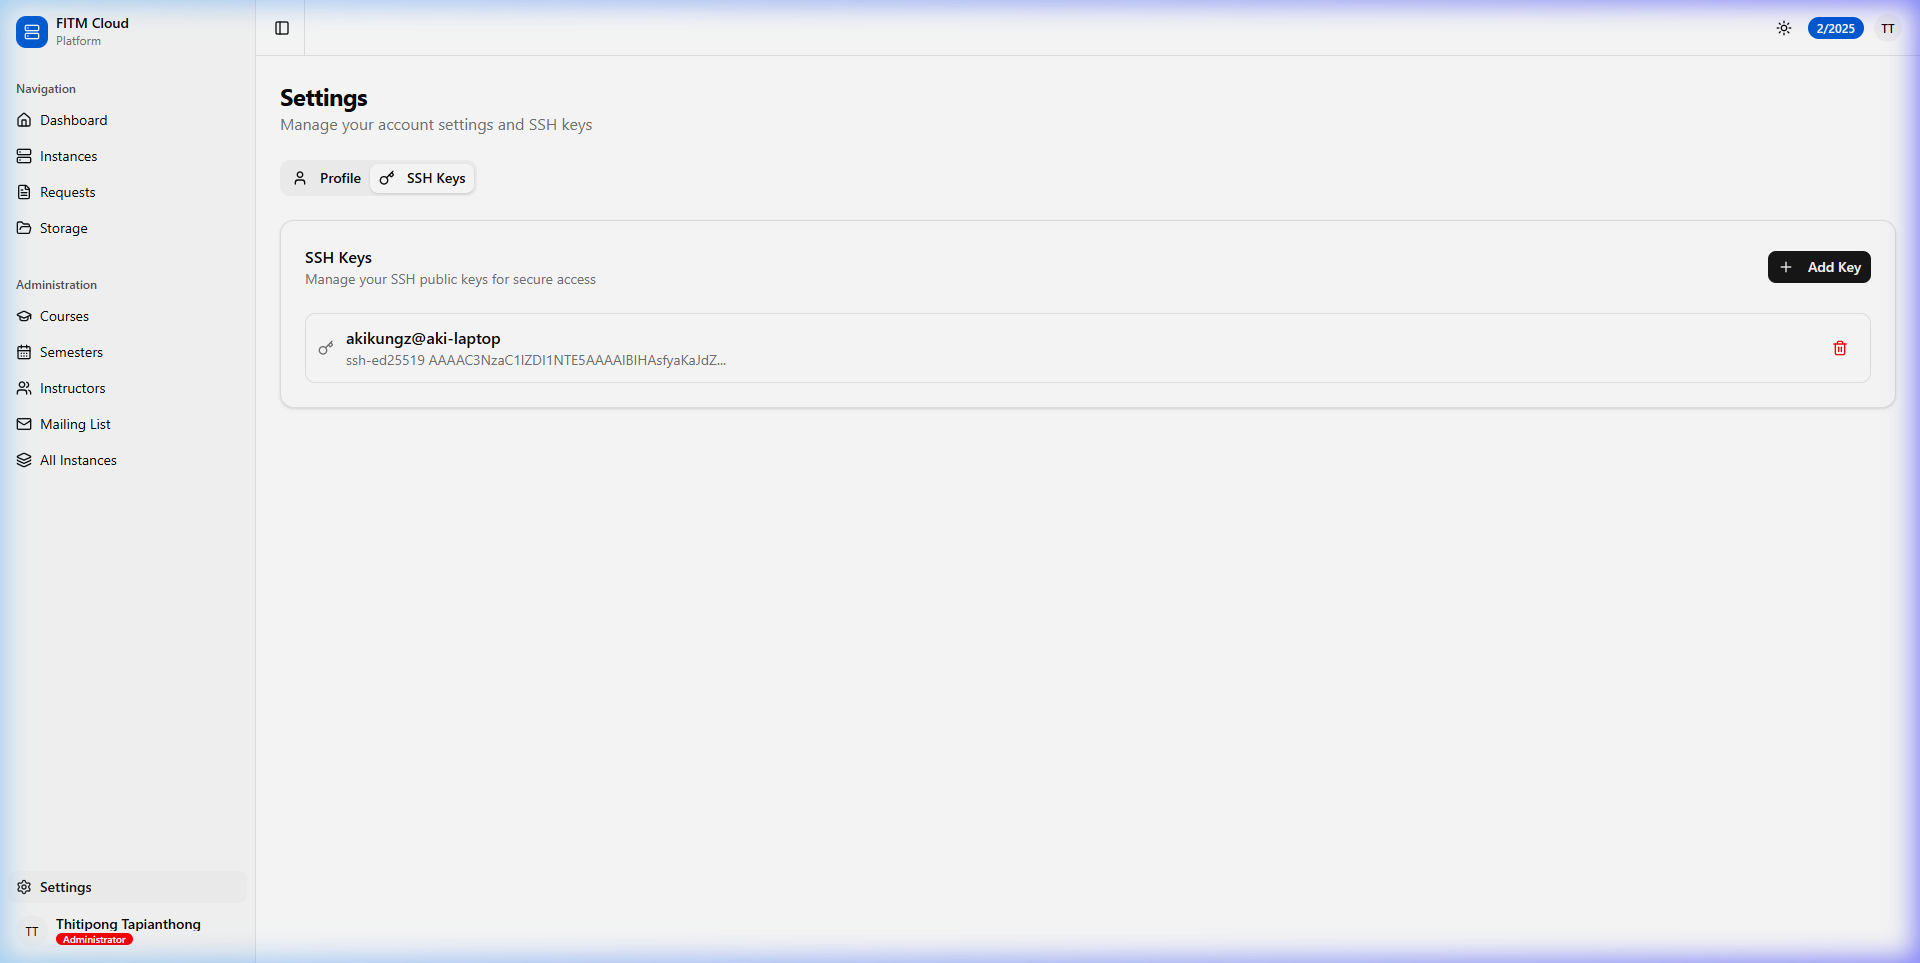
\includegraphics[width=\textwidth]{Image/web/dashboard/captured/ssh_keys.png}
}
\caption{\fontSixTeen{ภาพหน้าจอการเพิ่ม SSH Key ในเมนูการตั้งค่า (Settings)}} 
\label{figI:SshKeyPlaceholder}
\end{figure}

\begin{mycustomenum2}
    \item ไปที่ \textbf{Dashboard \textrightarrow Settings \textrightarrow SSH Keys \textrightarrow Add Key}
    \item วาง public key (ตัวอย่างเช่น \texttt{ssh-ed25519 AAAA...}) และตั้งชื่อให้จำง่าย
\end{mycustomenum2}

\vspace{0.5em}
\textbf{Connect to an instance}
\vspace{0.5em}

\hspace*{1.3em}
ในหน้ารายละเอียด instance ให้ดู \textbf{IP Address} และ \textbf{Default User} (หากแสดง)

\begin{figure}[H]
\centering
\adjustbox{frame, width=0.9\textwidth}{
    \begin{minipage}{0.85\textwidth}
        \texttt{\footnotesize
        ssh \textless username\textgreater@\textless ip-address\textgreater
        }
    \end{minipage}
}
\caption{\fontSixTeen{ตัวอย่างคำสั่ง SSH เพื่อเชื่อมต่อไปยัง instance}}
\label{figI:SshConnect}
\end{figure}

\hspace*{1.3em}
หากต้องระบุ private key ที่ไม่ใช่ค่า default

\begin{figure}[H]
\centering
\adjustbox{frame, width=0.9\textwidth}{
    \begin{minipage}{0.85\textwidth}
        \texttt{\footnotesize
        ssh -i \textasciitilde/.ssh/\textless private\_key\textgreater  \textless username\textgreater@\textless ip-address\textgreater
        }
    \end{minipage}
}
\caption{\fontSixTeen{ตัวอย่างการระบุ private key ตอนเชื่อมต่อ SSH}}
\label{figI:SshConnectWithKey}
\end{figure}

\vspace{0.5em}
\textbf{Notes about default password}
\vspace{0.5em}

\begin{mycustomenum2}
    \item หากใน UI แสดง default password ให้ถือเป็นข้อมูลอ่อนไหว
    \item ควรเปลี่ยนรหัสผ่านหลังเข้าใช้งานครั้งแรก (หาก image รองรับ)
    \item แนะนำให้ใช้ SSH key เป็นหลัก
\end{mycustomenum2}

\section{การตั้งค่า Reverse Proxy}
\hspace*{1.3em}
Reverse proxy ใช้สำหรับเปิดเผยบริการที่รันอยู่ภายใน VM (เช่น web app ที่พอร์ต 3000) ออกสู่ภายนอกผ่าน HTTP/HTTPS

\vspace{0.5em}
\textbf{Create a reverse proxy}
\vspace{0.5em}

\begin{figure}[H]
\centering
\adjustbox{frame, width=0.9\textwidth}{
    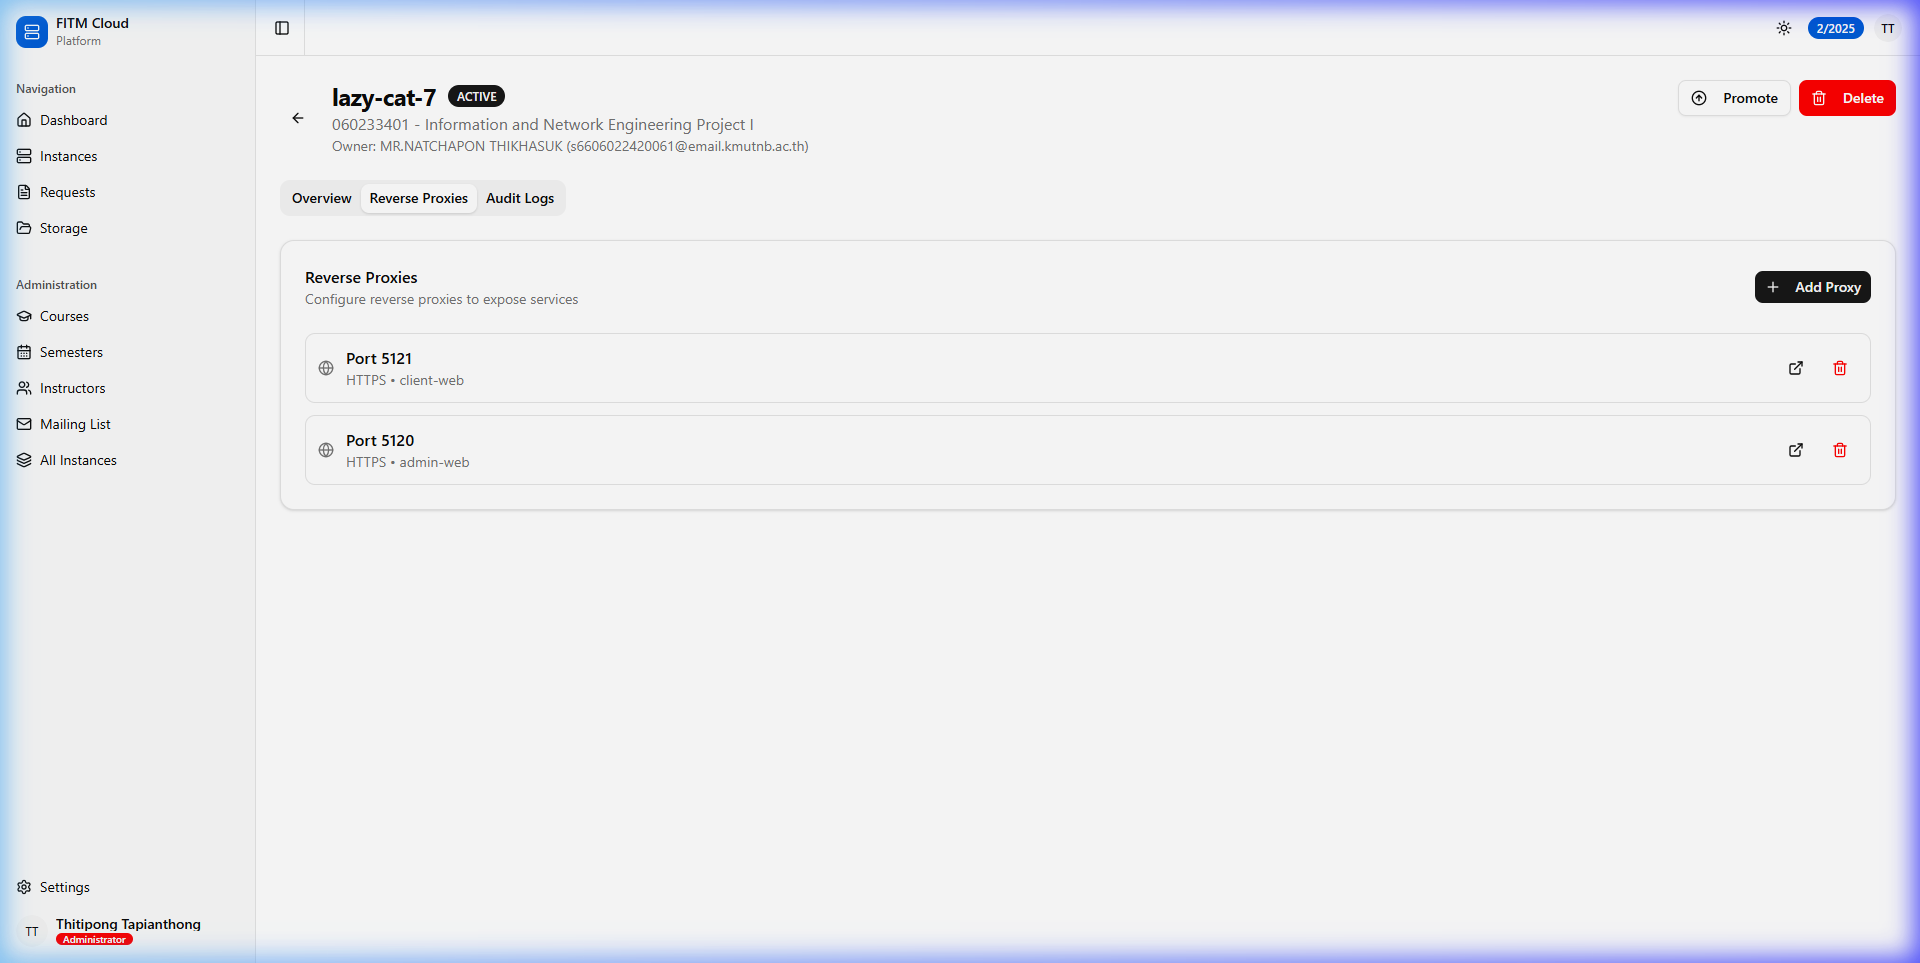
\includegraphics[width=\textwidth]{Image/web/dashboard/captured/reverse_proxies.png}
}
\caption{\fontSixTeen{ภาพหน้าจอการสร้างและกำหนดค่า Reverse Proxy}} 
\label{figI:ReverseProxyPlaceholder}
\end{figure}

\begin{mycustomenum2}
    \item ไปที่ \textbf{Dashboard \textrightarrow Instances \textrightarrow (select an instance) \textrightarrow Reverse Proxies}
    \item เพิ่ม proxy โดยระบุ:
    \begin{mycustomenum2}
        \item \textbf{Target port}: พอร์ตที่แอปของคุณฟังอยู่ใน VM (เช่น 3000)
        \item \textbf{Type}: HTTP หรือ HTTPS
        \item \textbf{Description} (ถ้ามี)
    \end{mycustomenum2}
\end{mycustomenum2}

\vspace{0.5em}
\textbf{Delete a reverse proxy}
\vspace{0.5em}

\begin{mycustomenum2}
    \item ลบ proxy ที่ไม่ใช้งานแล้วเพื่อลดความเสี่ยงการเปิดเผยบริการเกินจำเป็น
\end{mycustomenum2}

\section{การจัดการพื้นที่จัดเก็บไฟล์}
\hspace*{1.3em}
Storage เป็นหน้าเว็บสำหรับจัดการไฟล์และโฟลเดอร์ของผู้ใช้งาน

\begin{figure}[H]
\centering
\adjustbox{frame, width=0.9\textwidth}{
    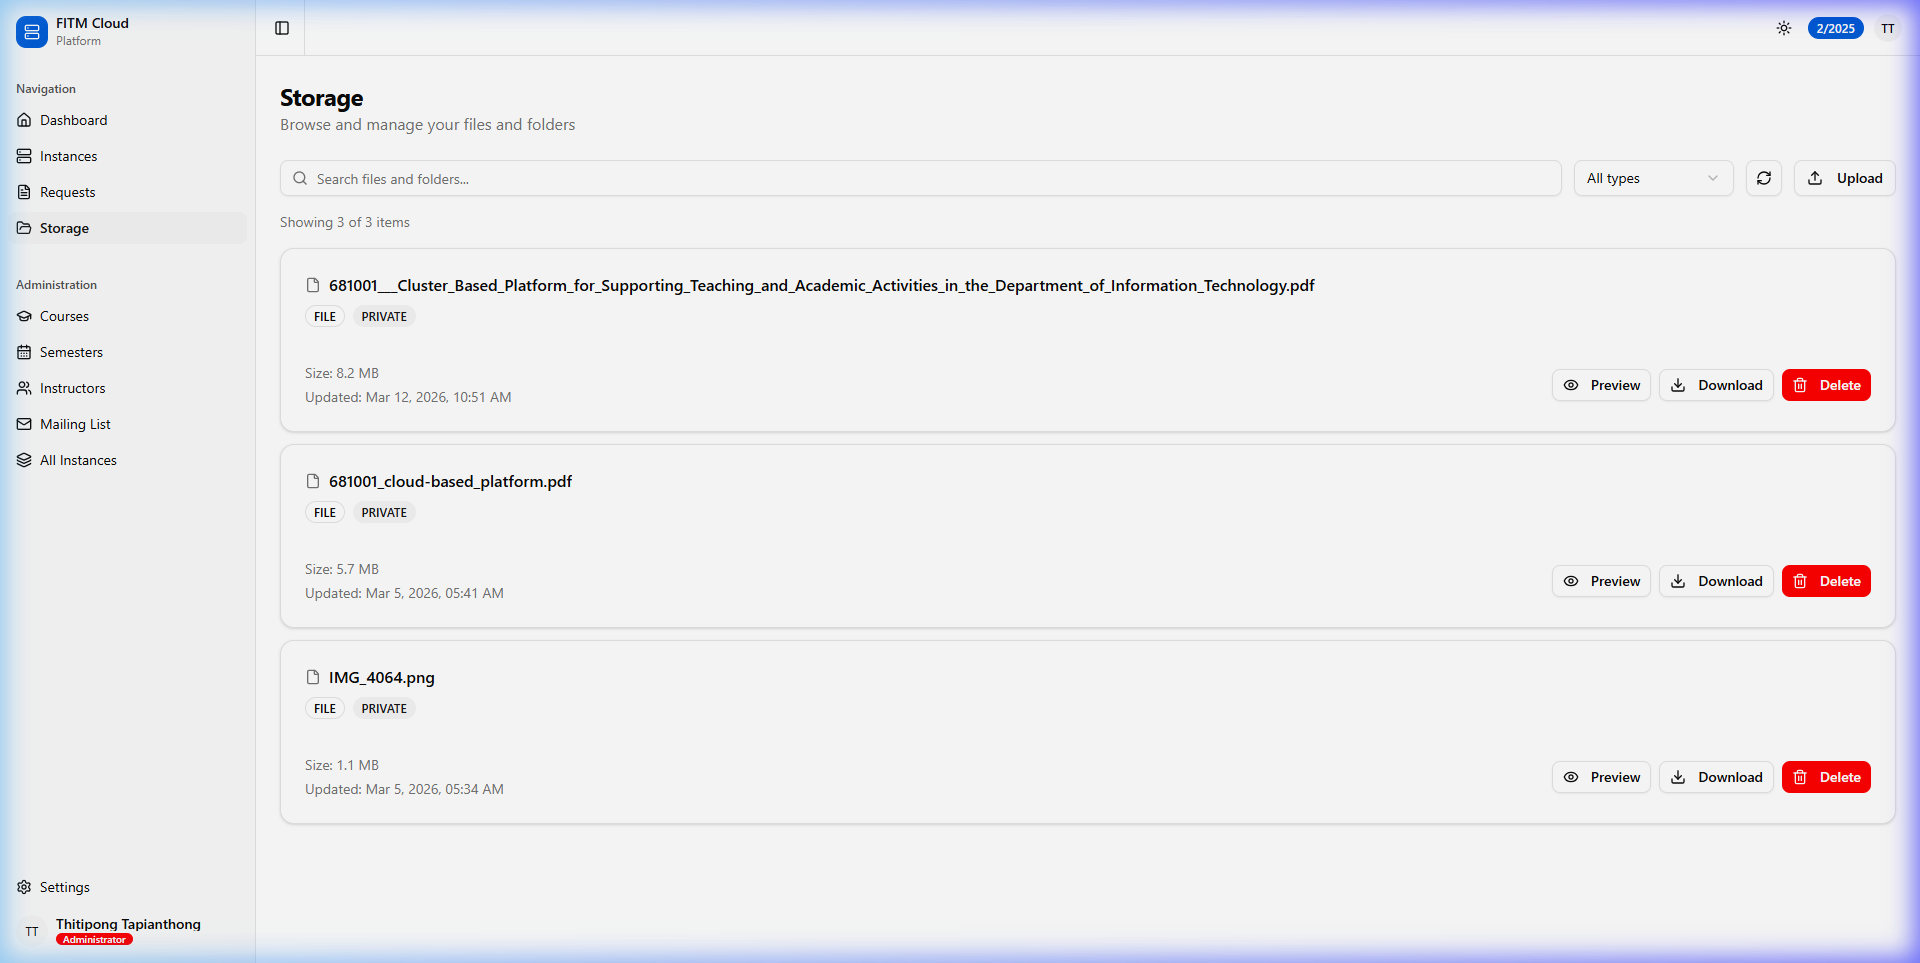
\includegraphics[width=\textwidth]{Image/web/dashboard/captured/storage.png}
}
\caption{\fontSixTeen{ภาพหน้าจอระบบการจัดการพื้นที่จัดเก็บไฟล์ (Storage)}} 
\label{figI:StoragePlaceholder}
\end{figure}

\begin{mycustomenum2}
    \item ไปที่ \textbf{Dashboard \textrightarrow Storage}
    \item Browse โฟลเดอร์ ดู preview ไฟล์ที่รองรับ (เช่น PDF) และจัดการไฟล์ตามที่ระบบรองรับ
\end{mycustomenum2}

\vspace{0.5em}
\textbf{Recommended practices}
\vspace{0.5em}

\begin{mycustomenum2}
    \item แยกโฟลเดอร์ตามรายวิชา/ภาคการศึกษาเพื่อให้ค้นหาได้ง่าย
    \item หลีกเลี่ยงการเก็บ secrets เช่น private key หรือ API token ใน storage
\end{mycustomenum2}

\section{การแก้ไขปัญหาเบื้องต้น}
\hspace*{1.3em}

\begin{figure}[H]
\centering
\adjustbox{frame, width=0.9\textwidth}{
    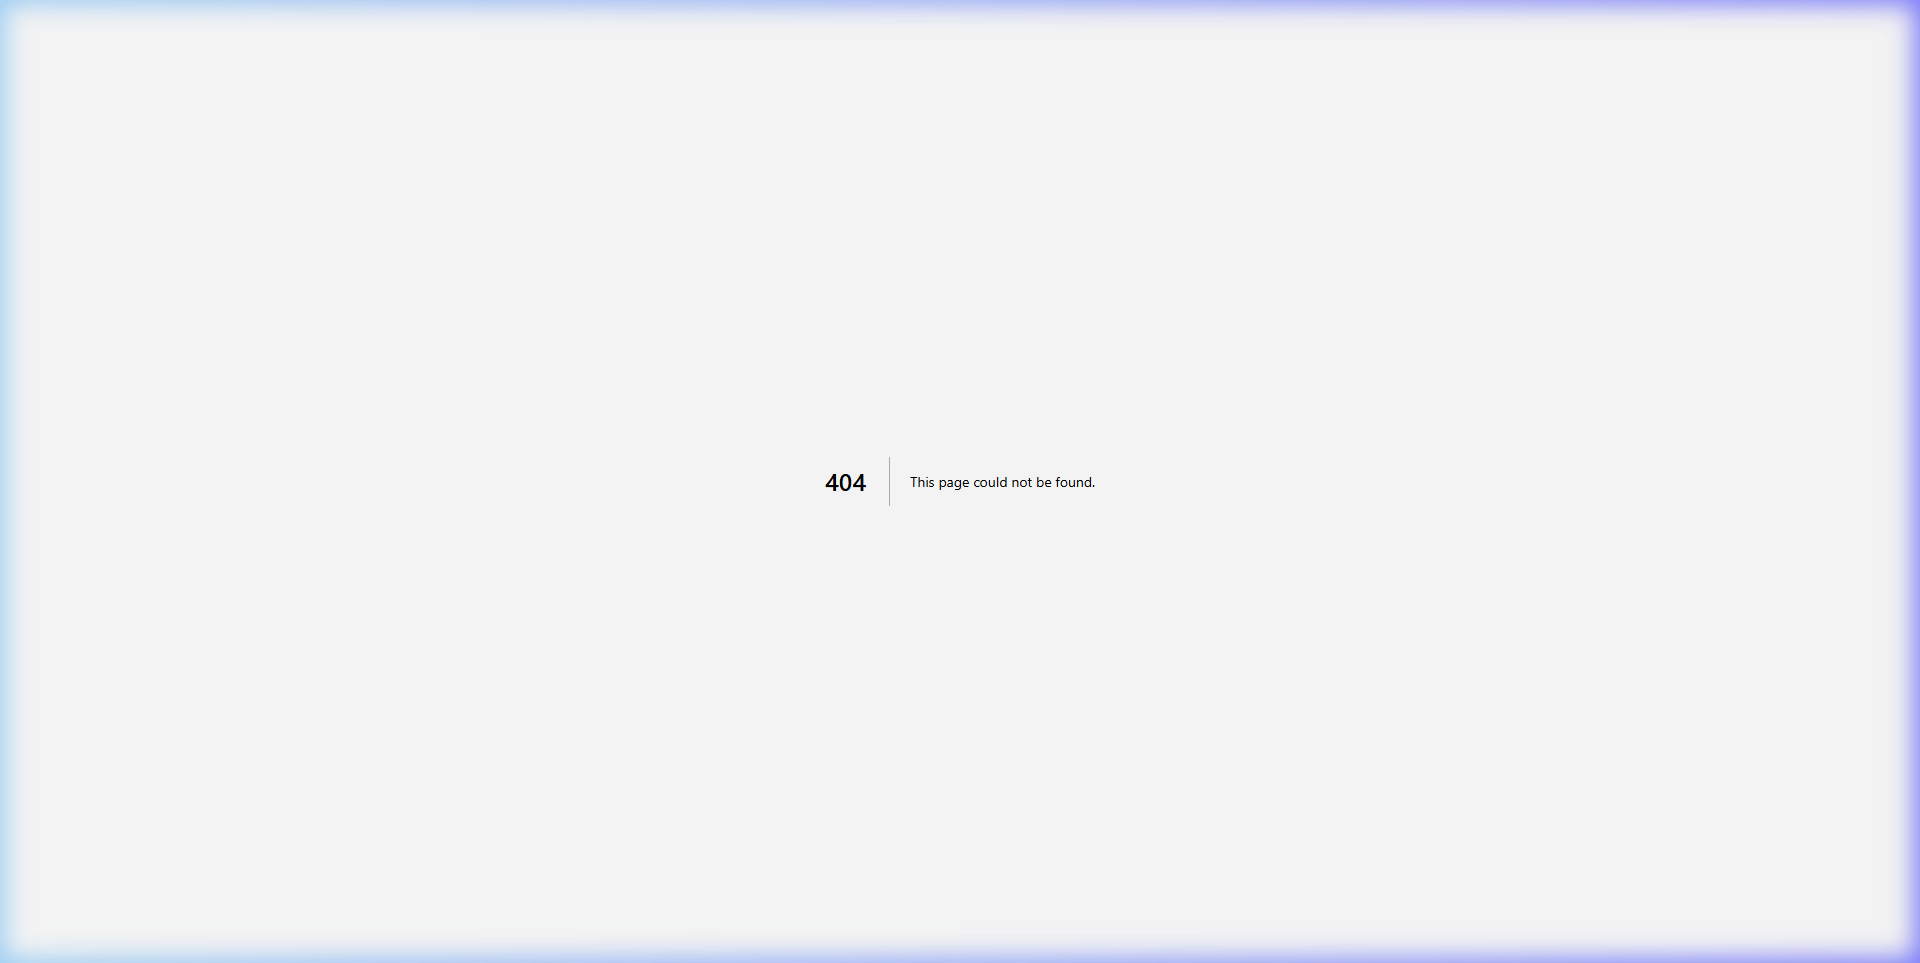
\includegraphics[width=\textwidth]{Image/web/dashboard/captured/troubleshoot.png}
}
\caption{\fontSixTeen{ภาพหน้าจอตัวอย่างระบบการแจ้งเตือนและการแก้ไขปัญหาเบื้องต้น}} 
\label{figI:TroubleshootPlaceholder}
\end{figure}

\vspace{0.5em}
\textbf{I can’t create a request}
\vspace{0.5em}

\begin{mycustomenum2}
    \item มักเกิดจาก role ไม่มี permission \textbf{CREATE\_REQUEST} หรือไม่มี course offerings ที่ active
    \item ตรวจสอบ role ใน \textbf{Settings} และติดต่อ admin หากข้อมูลบัญชีไม่ถูกต้อง
\end{mycustomenum2}

\vspace{0.5em}
\textbf{No Courses Available}
\vspace{0.5em}

\begin{mycustomenum2}
    \item ไม่มี course offerings ที่เปิดใช้งาน หรือบัญชีของผู้ใช้ไม่สามารถเห็นรายวิชาได้
    \item แนะนำให้ติดต่อผู้สอนหรือผู้ดูแลระบบ
\end{mycustomenum2}

\vspace{0.5em}
\textbf{Approved but no instance yet}
\vspace{0.5em}

\begin{mycustomenum2}
    \item การ provision เป็นงาน asynchronous ให้รอสักครู่และ refresh หน้า \textbf{Instances}
    \item หากค้างนานผิดปกติ ให้ผู้สอน/admin ตรวจสอบสถานะ request และระบบคิวเบื้องหลัง
\end{mycustomenum2}

\vspace{0.5em}
\textbf{SSH connection refused / timed out}
\vspace{0.5em}

\begin{mycustomenum2}
    \item ตรวจสอบว่า instance อยู่สถานะ \textbf{Active} และ IP Address ถูกต้อง
    \item ตรวจสอบว่าเพิ่ม SSH key แล้วใน \textbf{Settings \textrightarrow SSH Keys}
    \item หาก template หรือ firewall ปิด SSH ให้ติดต่อผู้สอน/admin
\end{mycustomenum2}

\vspace{0.5em}
\textbf{Can’t see reverse proxy / audit log tabs}
\vspace{0.5em}

\begin{mycustomenum2}
    \item role อาจไม่มี permission ที่เกี่ยวข้อง หรือ instance อยู่ในสถานะที่ feature ยังไม่พร้อม
\end{mycustomenum2}

\section{คำศัพท์สำคัญ}
\hspace*{1.3em}

\begin{mycustomenum2}
    \item \textbf{Instance}: เครื่องเสมือน (VM) ที่ระบบจัดสรรให้ผู้ใช้งาน/รายวิชา
    \item \textbf{Template}: OS image สำหรับสร้าง instance (เช่น Ubuntu, Debian)
    \item \textbf{Request}: คำขอสร้าง instance ที่ต้องผ่านการพิจารณา
    \item \textbf{Extended Request}: คำขอขยายอายุการใช้งานของ instance
    \item \textbf{Promote}: การกำหนดให้ instance เป็น long-term ตามนโยบาย
    \item \textbf{Reverse Proxy}: การแมป URL ภายนอกไปยังพอร์ตของบริการใน instance ผ่าน HTTP/HTTPS
\end{mycustomenum2}
